\chapter{Prezentacja warstwy użytkowej projektu}
\section{Opis aplikacji}
Aplikacja działa w trybie konsolowym. Po uruchomieniu następuje wczytanie danych z plików tekstowych, a następnie wyświetlenie głównego menu, które umożliwia:
\begin{itemize}
    \item Dodawanie produktów do magazynu,
    \item Realizację sprzedaży detalicznej (z automatycznym obliczaniem wydawanej reszty) oraz hurtowej (dla zarejestrowanych klientów),
    \item Rejestrację nowych klientów,
    \item Wyświetlanie listy produktów, klientów oraz historii zamówień.
\end{itemize}

\section{Przykładowe ekrany}
\subsection{Menu główne}
Widok głównego menu aplikacji. Użytkownik może wybrać jedną z dostępnych opcji: dodawanie produktu do magazynu, sprzedaż (detaliczną lub hurtową), rejestrację nowego klienta, wyświetlenie listy klientów i produktów, a także przegląd zamówień lub wyjście z programu.
\begin{figure}[ht]
    \centering
    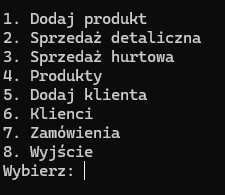
\includegraphics[width=0.5\linewidth]{figures/Menu.png}
    \caption{Menu Główne}
\end{figure}

\subsection{Dodawanie produktu}
Ekran służący do wprowadzania nowego produktu do magazynu. Użytkownik podaje nazwę produktu, cenę oraz ilość. Po poprawnym wprowadzeniu danych wyświetlany jest komunikat potwierdzający dodanie produktu.
\begin{figure}[ht]
    \centering
    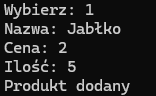
\includegraphics[width=0.5\linewidth]{figures/Dodawanie_pr.png}
    \caption{Dodawanie Produktów}
\end{figure}

\subsection{Sprzedaż detaliczna}
Widok obsługi sprzedaży detalicznej. Użytkownik wybiera produkt na podstawie ID, podaje ilość, a system automatycznie oblicza sumę do zapłaty. Następnie przyjmuje kwotę od klienta i w razie nadpłaty wylicza resztę. Transakcja zostaje zarejestrowana, a stany magazynowe są aktualizowane.
\begin{figure}[ht]
    \centering
    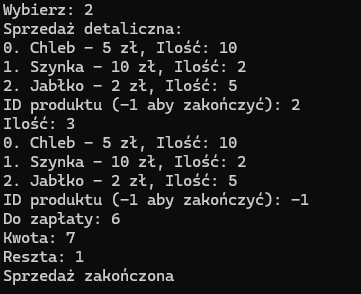
\includegraphics[width=0.5\linewidth]{figures/Spr_det.png}
    \caption{Sprzedaż detaliczna}
\end{figure}

\subsection{Sprzedaż hurtowa}
Ekran realizacji sprzedaży dla zarejestrowanych klientów. Po wprowadzeniu ID klienta, użytkownik wybiera produkty i ich ilości. Kwota za zakupy jest odejmowana od salda klienta, a magazyn zostaje zaktualizowany. Na końcu wyświetlany jest komunikat potwierdzający zakończenie transakcji.
\begin{figure}[ht]
    \centering
    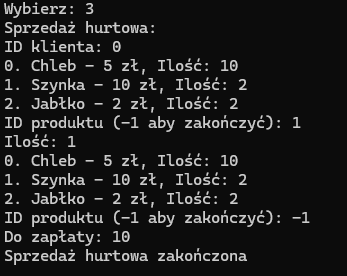
\includegraphics[width=0.5\linewidth]{figures/Spr_hur.png}
    \caption{Sprzedaż hurtowa}
\end{figure}

\subsection{Dodawanie klienta}
Okno pozwalające na dodanie nowego klienta do systemu. Użytkownik podaje imię, nazwisko i saldo portfela. Po wprowadzeniu danych klient jest zapisywany w bazie (plik tekstowy), a aplikacja informuje o poprawnym dodaniu klienta.
\begin{figure}[ht]
    \centering
    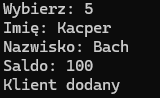
\includegraphics[width=0.5\linewidth]{figures/Dodaj_kl.png}
    \caption{Dodawanie klienta}
\end{figure}

\subsection{Wyświetlanie zamówień}
Widok prezentujący listę zamówień dokonanych w poprzednich sesjach oraz w bieżącej sesji. Każde zamówienie zawiera datę, dane klienta (lub informację o sprzedaży detalicznej), a także listę zakupionych produktów wraz z ich cenami i ilościami. Dzięki temu użytkownik może przejrzeć historię transakcji i sprawdzić szczegóły każdej sprzedaży.
\begin{figure}[ht]
    \centering
    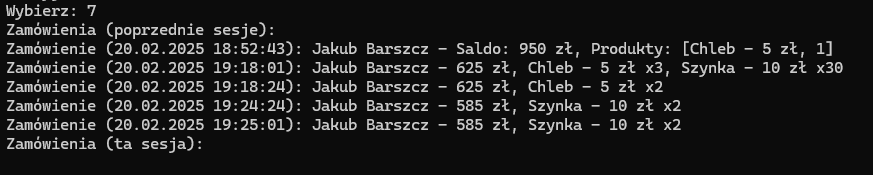
\includegraphics[width=0.9\linewidth]{figures/Zamowienia.png}
    \caption{Wyświetlanie Zamówień}
\end{figure}


